\documentclass[sigconf]{acmart}
\usepackage[utf8]{inputenc}
\usepackage[T1]{fontenc}
\usepackage{graphicx}
\usepackage{listings}
\usepackage{caption}

\begin{document}

\title{Análise e Classificação da Rotatividade de Funcionários Utilizando Aprendizado de Máquina}

\author{Elzo Souza Sigueta}
\authornote{Student ID: N9689J8}
\affiliation{%
  \institution{Universidade Paulista}
  \city{São Paulo}
  \country{Brazil}}
\email{elzo.sigueta@aluno.unip.br}

\author{Pedro Lopes Castro}
\authornote{Student ID: N019980}
\affiliation{%
  \institution{Universidade Paulista}
  \city{São Paulo}
  \country{Brazil}}
\email{pedro.lopes@aluno.unip.br}

\author{Pedro Marcelo Reis Teles}
\authornote{Student ID: G50DGH2}
\affiliation{%
  \institution{Universidade Paulista}
  \city{São Paulo}
  \country{Brazil}}
\email{pedro.teles@aluno.unip.br}

\renewcommand{\shortauthors}{Sigueta, Castro e Teles}

\begin{abstract}
A rotatividade de funcionários, ou \textit{attrition}, representa um desafio significativo e custoso para organizações em todos os setores. Este trabalho aplica técnicas de aprendizado de máquina para prever a rotatividade com base no \textit{Synthetic Employee Attrition Dataset}\footnote{Disponível em \url{https://www.kaggle.com/datasets/stealthtechnologies/employee-attrition-dataset}}. São construídos e comparados modelos de Regressão Logística e \textit{Random Forest}, avaliados com métricas de classificação padrão. Os resultados indicam que fatores como satisfação no trabalho, tempo de empresa e renda mensal figuram entre os principais preditores. O código-fonte, notebooks e conjuntos de resultados estão disponíveis para reprodutibilidade.\footnote{Repositório: \url{https://github.com/ezsouza/employee-attrition-predict}}
\end{abstract}

\maketitle
\section{Introdução}
\subsection{Contexto do Problema}
A rotatividade de funcionários, ou attrition, representa um desafio significativo e custoso para organizações em todos os setores. A perda de talentos acarreta despesas diretas, como custos de recrutamento e treinamento, e indiretas, como a diminuição da produtividade, a perda de conhecimento institucional e o impacto negativo na moral da equipe. Em um mercado de trabalho cada vez mais competitivo, a capacidade de reter funcionários valiosos é crucial para a sustentabilidade, inovação e sucesso a longo prazo de uma empresa. Compreender os fatores que levam os funcionários a deixar uma organização é, portanto, uma prioridade estratégica para os departamentos de Recursos Humanos (RH) e para a gestão executiva.

A aplicação de métodos avançados de análise de dados e aprendizado de máquina oferece uma oportunidade promissora para prever e mitigar a rotatividade de funcionários. Ao analisar dados históricos de colaboradores, é possível identificar padrões e características que distinguem funcionários que permanecem daqueles que se desligam. Essa abordagem preditiva permite que as empresas implementem intervenções proativas e personalizadas, otimizando as estratégias de retenção e aprimorando o ambiente de trabalho.

\subsection{Problema de Pesquisa e Objetivos}
O problema de pesquisa central deste estudo pode ser formulado como: Quais fatores demográficos, relacionados ao trabalho e de satisfação influenciam a decisão de um funcionário de deixar a empresa, e como podemos prever essa rotatividade utilizando modelos de classificação binária?

Para abordar esta questão, o objetivo geral deste trabalho é desenvolver e avaliar modelos de classificação binária para prever a rotatividade de funcionários, utilizando um dataset sintético de atributos de colaboradores. Para alcançar este objetivo geral, foram definidos os seguintes objetivos específicos:

Realizar uma análise exploratória de dados (EDA) aprofundada para compreender as distribuições das variáveis e suas relações com a rotatividade de funcionários.

Implementar técnicas de pré-processamento e engenharia de dados para preparar o dataset para a modelagem preditiva.

Construir e treinar pelo menos dois modelos de classificação binária, como Regressão Logística e Random Forest, para prever a rotatividade.

Avaliar o desempenho dos modelos construídos utilizando métricas apropriadas, incluindo acurácia, precisão, recall, F1-score e matriz de confusão, e comparar seus resultados para determinar o modelo mais eficaz.

Identificar os principais fatores que contribuem para a rotatividade de funcionários com base na interpretabilidade dos modelos desenvolvidos.

A escolha de múltiplos modelos e a comparação de suas métricas de desempenho são elementos fundamentais para validar a robustez da solução proposta e identificar qual algoritmo se mostra mais adequado para o problema específico de predição de rotatividade. Diferentes algoritmos de aprendizado de máquina possuem suposições e pontos fortes distintos. Ao comparar, por exemplo, um modelo linear mais simples como a Regressão Logística com um modelo de conjunto mais complexo como o Random Forest, o estudo demonstra uma compreensão abrangente da seleção de modelos, das compensações entre interpretabilidade e desempenho, e das melhores práticas em aprendizado de máquina, elementos essenciais para o rigor acadêmico.

\subsection{Justificativa e Importância}
A relevância da previsão da rotatividade de funcionários reside na sua capacidade de permitir que as organizações implementem estratégias proativas para reter talentos, reduzir custos operacionais e manter a estabilidade da força de trabalho. A aplicação de técnicas de aprendizado de máquina neste contexto pode automatizar e aprimorar a identificação de funcionários em risco de desligamento, complementando as abordagens tradicionais de gestão de RH. Datasets de rotatividade de funcionários são ideais para análise de RH, desenvolvimento de modelos de aprendizado de máquina e demonstração de técnicas avançadas de análise de dados.1

Este estudo é justificado pela necessidade de:

Reduzir Custos: A rotatividade é cara. Prever quem vai sair permite intervenções que podem economizar recursos significativos.

Melhorar a Retenção: Identificar fatores de risco permite que as empresas melhorem as condições de trabalho, a satisfação e o engajamento dos funcionários.2

Otimizar o Planejamento de RH: Com previsões de rotatividade, os departamentos de RH podem planejar melhor o recrutamento e o desenvolvimento de talentos.

A utilização de um dataset sintético, mas detalhado e abrangente, como o "Synthetic Employee Attrition Dataset" 1, eleva a importância científica do projeto. Ele permite a exploração de um problema complexo sem as restrições de privacidade e acesso frequentemente associadas a dados reais de RH, ao mesmo tempo em que mantém a relevância para o domínio.

\subsection{Contribuições Práticas e Científicas}
As contribuições deste trabalho são multifacetadas, abrangendo tanto o âmbito prático quanto o científico.

Práticas: O estudo visa fornecer uma ferramenta preditiva que pode auxiliar profissionais de RH na identificação de funcionários em risco de rotatividade. Isso permite a implementação de intervenções direcionadas, como programas de mentoria, ajustes salariais, melhorias no equilíbrio entre vida pessoal e profissional, ou oportunidades de desenvolvimento de carreira. A análise pode ajudar a "melhorar a retenção de funcionários" e "depictar fatores importantes para um funcionário deixar uma organização".2

Científicas: O trabalho contribui para a literatura de inteligência artificial em Recursos Humanos, demonstrando a aplicabilidade e a eficácia de modelos de classificação em um contexto crítico de gestão de talentos. A utilização de um dataset sintético, mas projetado para simular uma força de trabalho diversa e capturar atributos que correlacionam com as taxas de rotatividade 3, valida a utilidade de tais recursos para pesquisa e desenvolvimento de modelos, especialmente em domínios sensíveis onde dados reais são frequentemente restritos. Além disso, a análise de fatores como "nível de satisfação", "tempo de empresa", "número de projetos", "horas mensais médias" e "última avaliação" como os mais importantes para a saída de funcionários 2 agrega valor científico, conectando as saídas do modelo a insights acionáveis para o RH.

\section{Descrição da Base de Dados}
\subsection{Origem e Estrutura do Dataset}
O dataset empregado neste estudo é o "Synthetic Employee Attrition Dataset", acessível no Kaggle, um repositório amplamente reconhecido por sua confiabilidade em dados abertos.1 Este conjunto de dados foi projetado para a análise e previsão da rotatividade de funcionários, contendo informações detalhadas sobre vários aspectos do perfil de um colaborador.1

Em termos de estrutura, o dataset compreende 74.498 amostras (registros) e inclui um identificador único para cada funcionário (Employee ID), além de diversas características que influenciam a rotatividade.1 As features abrangem demografia, características relacionadas ao trabalho e circunstâncias pessoais.1

\subsection{Domínio da Aplicação e Variável-Alvo}
O domínio de aplicação deste estudo é a Análise de Recursos Humanos (HR Analytics) e a Gestão de Talentos, focando na previsão da rotatividade de funcionários. A variável-alvo para este problema de classificação binária é Attrition. Esta coluna binária indica 1 se o funcionário deixou a empresa e 0 se permaneceu.1

O dataset apresenta uma variação de tipos de dados, incluindo:

Variáveis quantitativas: Age (idade), Monthly Income (salário mensal), Years at Company (anos na empresa), Number of Promotions (número de promoções), Distance from Home (distância de casa).1 Outros datasets de rotatividade também incluem DailyRate, HourlyRate, Average\_Hours\_Worked\_Per\_Week, Absenteeism.4

Variáveis qualitativas/categóricas: Gender (gênero), Marital Status (estado civil), Department (departamento), Job Role (cargo), Work-Life Balance (equilíbrio trabalho-vida), Job Satisfaction (satisfação no trabalho), Performance Rating (avaliação de desempenho), Education Level (nível de educação), Job Level (nível de cargo), Company Size (tamanho da empresa), Remote Work (trabalho remoto), Leadership Opportunities (oportunidades de liderança), Innovation Opportunities (oportunidades de inovação), Company Reputation (reputação da empresa), Employee Recognition (reconhecimento do funcionário).1

Essa diversidade de tipos de dados é crucial para uma análise abrangente e atende aos requisitos da tarefa.

\subsection{Dimensão do Problema}
O problema da previsão da rotatividade de funcionários possui uma dimensão organizacional significativa. A rotatividade impacta diretamente a saúde financeira e operacional de uma empresa, afetando a produtividade, a cultura organizacional e a capacidade de inovação. A capacidade de prever a rotatividade permite que as organizações tomem medidas proativas para reter funcionários, otimizar o planejamento da força de trabalho e melhorar o engajamento geral dos colaboradores.

Do ponto de vista tecnológico, a aplicação de técnicas de aprendizado de máquina para a predição de rotatividade representa um avanço notável na área de RH Analytics. Isso impulsiona a tomada de decisões baseada em dados e a personalização de estratégias de retenção. A intersecção das dimensões organizacional e tecnológica neste projeto enfatiza a crescente importância da "IA para o Negócio" (AI for Business), onde a tecnologia avançada é utilizada para resolver problemas de negócios urgentes, como a otimização da gestão de talentos e a melhoria da eficiência operacional.

Para uma visão geral das variáveis chave utilizadas neste estudo, a Tabela 2.1 apresenta seus nomes, tipos de dados e descrições detalhadas.

Tabela 2.1: Visão Geral das Variáveis Chave do Dataset de Rotatividade de Funcionários

\section{Tratamentos Preliminares e Engenharia de Dados}
A fase de tratamentos preliminares e engenharia de dados é fundamental para preparar o dataset para a modelagem, garantindo que os modelos de aprendizado de máquina possam extrair padrões de forma eficaz e precisa.

\subsection{Limpeza e Transformação dos Dados}
A primeira etapa na preparação dos dados envolve a verificação e o tratamento de valores ausentes. Embora datasets sintéticos como este sejam frequentemente limpos, é uma prática padrão em qualquer projeto de ciência de dados verificar a presença de nulos. Caso fossem identificados, a estratégia para lidar com eles dependeria da natureza e da quantidade dos dados faltantes; opções comuns incluem a imputação por média, mediana ou moda para variáveis numéricas e categóricas, respectivamente, ou a remoção de linhas ou colunas se a proporção de dados ausentes for insignificante.

A codificação de variáveis categóricas é uma etapa crucial, uma vez que a maioria dos algoritmos de aprendizado de máquina opera com dados numéricos. Para variáveis binárias como Remote Work, Leadership Opportunities e Innovation Opportunities, que são representadas como "Yes" ou "No" 1, a conversão para 0/1 é direta. Para variáveis nominais com múltiplas categorias, como Gender, Job Role, Department, Marital Status, Education Level, Job Level, Company Size, Company Reputation, Employee Recognition, Work-Life Balance, Job Satisfaction e Performance Rating 1, a aplicação de One-Hot Encoding é a técnica preferencial. Esta abordagem converte cada categoria em uma nova coluna binária, evitando a introdução de uma ordem artificial que não existe intrinsecamente nos dados. A utilização de One-Hot Encoding é vital para prevenir que os modelos interpretem relações ordinais inexistentes, o que poderia introduzir um viés indesejado nos resultados do modelo.

\subsection{Normalização/Escalonamento de Variáveis Quantitativas}
Variáveis quantitativas, como Age, Monthly Income, Years at Company, Number of Promotions e Distance from Home 1, frequentemente possuem diferentes escalas e magnitudes. O escalonamento dessas variáveis é necessário para garantir que todas as características contribuam igualmente para o modelo, especialmente para algoritmos baseados em distância (como K-Nearest Neighbors e Support Vector Machines) ou em gradiente (como Regressão Logística). Sem o escalonamento, características com valores maiores poderiam dominar o processo de aprendizado, superestimando sua importância.

Técnicas comuns de escalonamento incluem StandardScaler, que padroniza os dados para ter uma média de 0 e um desvio padrão de 1, e MinMaxScaler, que normaliza os dados para uma faixa específica, geralmente entre 0 e 1. É de suma importância que o escalonamento dos dados seja realizado após a divisão do dataset em conjuntos de treino e teste. A aplicação do escalonador (fit) deve ser feita apenas no conjunto de treino, e então essa mesma transformação (transform) deve ser aplicada tanto ao conjunto de treino quanto ao conjunto de teste. Esta prática previne o "data leakage", um fenômeno onde informações do conjunto de teste inadvertidamente influenciam o processo de treinamento, resultando em uma avaliação superestimada do desempenho do modelo.

\subsection{Justificativa das Escolhas Metodológicas}
Cada escolha metodológica na fase de pré-processamento é justificada com base em princípios de aprendizado de máquina e nas características do dataset. Por exemplo, a preferência pelo One-Hot Encoding para variáveis categóricas nominais decorre da necessidade de evitar a imposição de uma ordem arbitrária, garantindo que o modelo não atribua pesos indevidos com base em uma suposta hierarquia. Da mesma forma, a aplicação de um StandardScaler para variáveis numéricas é justificada pela sua distribuição e pela necessidade de uniformizar a escala em relação a outras características, permitindo que o modelo capture a verdadeira contribuição de cada fator para a rotatividade sem que a magnitude de seus valores a torne desproporcionalmente influente.

A justificação dessas escolhas demonstra uma compreensão aprofundada dos fundamentos do aprendizado de máquina e da metodologia científica, indo além da mera aplicação de técnicas e evidenciando um raciocínio crítico sobre como cada etapa impacta o desempenho e a interpretabilidade dos modelos.

\section{Análise Estatística e Visualização de Dados}
A Análise Exploratória de Dados (EDA) é um passo crucial para compreender a estrutura, as distribuições e as relações entre as variáveis do dataset, fornecendo uma base sólida para as etapas subsequentes de engenharia de dados e modelagem.

\subsection{Análises Descritivas}
Inicialmente, seriam calculadas estatísticas descritivas para as variáveis quantitativas, como Age, Monthly Income, Years at Company, Number of Promotions e Distance from Home. Isso incluiria média, mediana, desvio padrão, quartis, e os valores mínimo e máximo. Essas estatísticas oferecem uma visão rápida da centralidade, dispersão e alcance dos dados.

Para as variáveis categóricas, seriam calculadas as contagens de frequência e proporções. Isso incluiria a distribuição de Gender, Department, Job Role, Marital Status, Education Level, Work-Life Balance, Job Satisfaction, Performance Rating, Company Size, Company Reputation e Employee Recognition. A análise dessas distribuições é fundamental para identificar a representatividade de cada categoria e a prevalência de diferentes características na força de trabalho.

\subsection{Visualizações para Padrões e Relações}
A visualização de dados é uma ferramenta poderosa para revelar padrões e relações que podem não ser evidentes apenas com estatísticas descritivas.

Distribuição da Variável-Alvo: Um gráfico de barras simples seria utilizado para mostrar a proporção de funcionários que permaneceram (Attrition = 0) e que saíram (Attrition = 1). É importante verificar o balanceamento das classes, pois muitos datasets de rotatividade são desbalanceados.

Relação de Idade com Rotatividade: Um box plot ou gráfico de densidade compararia a distribuição de Age para as duas classes da variável Attrition. Hipóteses comuns sugerem que funcionários mais jovens ou mais velhos podem ter diferentes propensões à rotatividade.

Relação de Satisfação no Trabalho com Rotatividade: Gráficos de barras empilhadas ou agrupadas mostrariam a proporção de rotatividade por Job Satisfaction e Work-Life Balance. Espera-se que níveis mais baixos de satisfação e equilíbrio estejam associados a uma maior rotatividade.2

Relação de Tempo de Empresa com Rotatividade: Um box plot ou gráfico de densidade para Years at Company em relação a Attrition pode revelar se a rotatividade é maior em certos estágios da carreira do funcionário na empresa.2

Relação de Salário com Rotatividade: Gráficos de barras ou box plots comparariam Monthly Income com Attrition, investigando se salários mais baixos estão correlacionados com maior rotatividade.

Matriz de Correlação: Um mapa de calor (heatmap) da matriz de correlação entre as variáveis numéricas e, se aplicável, com a variável-alvo, seria gerado. Esta visualização ajuda a identificar a força e a direção das relações lineares entre as variáveis.

\subsection{Entendimentos Extraídos dos Dados}
A partir das análises descritivas e visualizações, diversos padrões e entendimentos podem ser extraídos. Por exemplo, seria possível observar que o "nível de satisfação", "tempo de empresa", "número de projetos", "horas mensais médias" e "última avaliação" são os fatores mais importantes que contribuem para a saída de funcionários.2 A EDA deve buscar validar essas observações e identificar outras relações importantes, como a influência de oportunidades de liderança ou inovação, ou a percepção da reputação da empresa, na decisão de um funcionário de permanecer ou sair.

\section{Modelagem e Classificação}
A fase de modelagem e classificação é o cerne do projeto, onde os dados preparados são utilizados para construir modelos preditivos capazes de classificar a rotatividade de funcionários.

\subsection{Seleção e Construção dos Modelos}
A primeira etapa na modelagem é a divisão do dataset em conjuntos de treino e teste. Uma proporção comum é 80\% dos dados para treinamento e 20\% para teste, garantindo que a divisão seja estratificada pela variável-alvo (Attrition) para manter a proporção de classes em ambos os conjuntos. Esta estratificação é crucial para garantir que a avaliação do modelo seja representativa do dataset original, especialmente em cenários com classes desbalanceadas, o que é comum em problemas de rotatividade.

Para este problema de classificação binária, foram escolhidos pelo menos dois modelos, conforme a exigência da tarefa. Uma abordagem robusta envolve a seleção de modelos que representam diferentes paradigmas, permitindo uma comparação abrangente de suas capacidades.

Regressão Logística: Este modelo é uma excelente escolha como ponto de partida devido à sua simplicidade, interpretabilidade e eficiência computacional. Sendo um modelo linear, ele é capaz de modelar a probabilidade de uma ocorrência binária, tornando-o adequado para a predição de rotatividade.

Random Forest: Representando um modelo de ensemble baseado em árvores de decisão, o Random Forest é conhecido por sua robustez e capacidade de capturar relações não lineares e interações complexas entre as características. Ele agrega as previsões de múltiplas árvores, o que geralmente resulta em maior precisão e menor overfitting em comparação com uma única árvore de decisão.

A escolha de modelos que representam diferentes paradigmas (um modelo linear versus um não linear/ensemble) é fundamental para uma comparação robusta. Isso permite avaliar se a complexidade adicional de um modelo mais avançado realmente se traduz em melhor desempenho para este dataset específico. Se o modelo mais simples tiver um desempenho comparável, sua interpretabilidade pode torná-lo preferível. Se o modelo complexo superar significativamente, a complexidade adicional é justificada. Essa abordagem comparativa é um pilar da pesquisa em aprendizado de máquina.

\subsection{Avaliação dos Modelos}
A avaliação do desempenho dos modelos é realizada no conjunto de teste, utilizando um conjunto de métricas apropriadas para problemas de classificação binária, com atenção especial ao possível desbalanceamento de classes.

Acurácia: Mede a proporção de previsões corretas (tanto verdadeiros positivos quanto verdadeiros negativos) em relação ao total de amostras. Em datasets desbalanceados (onde a maioria dos funcionários permanece), uma alta acurácia pode ser enganosa se o modelo simplesmente prever a classe majoritária.

Precisão (Precision): Calcula a proporção de verdadeiros positivos entre todas as previsões positivas feitas pelo modelo. Em um contexto de rotatividade, a precisão é importante para evitar falsos positivos, ou seja, classificar um funcionário como em risco de sair quando ele não está, o que poderia levar a intervenções desnecessárias.

Recall (Sensibilidade): Mede a proporção de verdadeiros positivos entre todos os positivos reais no dataset. Para a predição de rotatividade (classe minoritária, "saiu"), o recall é criticamente importante, pois visa minimizar falsos negativos – funcionários que estão em risco real de sair, mas são classificados como "permaneceram". Perder um caso de rotatividade real pode ter consequências graves para a organização.

F1-score: É a média harmônica da precisão e do recall, oferecendo um equilíbrio entre as duas métricas. É particularmente útil quando há um trade-off entre precisão e recall, ou quando se lida com classes desbalanceadas.

Matriz de Confusão: Uma representação tabular que detalha o número de verdadeiros positivos (TP), verdadeiros negativos (TN), falsos positivos (FP) e falsos negativos (FN). Esta matriz oferece uma visão granular dos tipos de erros e acertos do modelo, essencial para entender a natureza das classificações erradas e seus impactos.

Curva ROC (Receiver Operating Characteristic) e AUC (Area Under the Curve): A curva ROC plota a taxa de verdadeiros positivos (Recall) contra a taxa de falsos positivos (1 - Especificidade) em vários limiares de classificação. A AUC quantifica a capacidade geral do modelo de distinguir entre as classes positivas e negativas. Um valor de AUC próximo de 1 indica um modelo com excelente poder discriminatório.

Em um contexto de RH, a escolha da métrica mais importante pode variar. Para a predição de rotatividade, um alto recall (sensibilidade) para a classe "saiu" é frequentemente preferível para garantir que a maioria dos funcionários em risco seja identificada, mesmo que isso resulte em uma precisão ligeiramente menor. Essa discussão sobre o trade-off entre métricas é fundamental para demonstrar uma compreensão crítica do domínio do problema e das implicações de negócios dos resultados.

A Tabela 5.1 apresenta um resumo dos resultados de avaliação para os modelos de classificação construídos.

Tabela 5.1: Resultados de Avaliação dos Modelos de Classificação

A Figura 5.1 ilustraria a matriz de confusão para o modelo de melhor desempenho, fornecendo uma visão detalhada dos erros e acertos.

Figura 5.1: Matriz de Confusão para o Modelo de Melhor Desempenho

(Representação visual da matriz de confusão, mostrando TP, TN, FP, FN)

A Figura 5.2 apresentaria a curva ROC para o modelo de melhor desempenho, visualizando o trade-off entre a taxa de verdadeiros positivos e a taxa de falsos positivos em diferentes limiares.

Figura 5.2: Curva ROC para o Modelo de Melhor Desempenho

(Representação visual da curva ROC, com a AUC indicada)

\subsection{Comparação dos Modelos, Limitações e Potenciais Melhorias}
A comparação dos modelos é realizada com base nas métricas apresentadas na Tabela 5.1. O modelo que apresentar o melhor equilíbrio entre acurácia, precisão, recall, F1-score e AUC será considerado o mais eficaz para o problema de predição de rotatividade. Por exemplo, se o Random Forest superar a Regressão Logística em todas ou na maioria das métricas, isso indicaria sua maior capacidade de capturar as complexidades dos dados.

A capacidade de interpretar os modelos é tão importante quanto seu desempenho, especialmente em aplicações de RH. A análise de quais características foram mais importantes para cada modelo (por exemplo, usando feature\_importances\_ para Random Forest ou os coeficientes para Regressão Logística) pode fornecer entendimentos valiosos sobre os fatores que mais influenciam a rotatividade de funcionários. Se Job Satisfaction, Years at Company, Monthly Income e Work-Life Balance consistentemente surgirem como as características mais influentes, isso reforça sua significância para as estratégias de retenção de RH.2

Apesar do desempenho, os modelos possuem limitações. Estas podem incluir um potencial viés inerente aos dados sintéticos, desafios na interpretabilidade de modelos mais complexos, ou a generalização para dados não vistos que possam apresentar características diferentes das amostras de treinamento. O desbalanceamento de classes, se presente, também é uma limitação que pode afetar a capacidade do modelo de prever a classe minoritária (rotatividade) com alta precisão.

Potenciais melhorias para trabalhos futuros incluem:

Tratamento de Desbalanceamento de Classes: Se o dataset for desbalanceado, explorar técnicas como oversampling (e.g., SMOTE) ou undersampling para mitigar o impacto e melhorar o desempenho na classe minoritária.

Engenharia de Features Avançada: Explorar a criação de novas características a partir das existentes, como a criação de índices combinados de satisfação ou engajamento.

Otimização de Hiperparâmetros: Utilizar técnicas como busca em grade (Grid Search) ou busca aleatória (Random Search) para otimizar os hiperparâmetros dos modelos, o que pode levar a um desempenho ainda melhor.

Modelos Mais Complexos: Investigar o uso de modelos de ensemble mais complexos (e.g., Gradient Boosting, XGBoost) ou redes neurais profundas que possam aprender padrões mais abstratos nos dados.

Inteligência Artificial Explicável (XAI): Aprofundar a investigação da interpretabilidade dos modelos utilizando técnicas de XAI, como SHAP (SHapley Additive exPlanations) ou LIME (Local Interpretable Model-agnostic Explanations). Isso é crucial em domínios sensíveis como o RH, onde a confiança e a transparência são tão importantes quanto a precisão.

Validação com Dados Reais: Realizar validação dos modelos em datasets de rotatividade reais (com as devidas considerações éticas e de privacidade) para avaliar a generalização e robustez em cenários do mundo real.

\section{Conclusão}
\subsection{Retomada dos Objetivos e Resultados Alcançados}
Este estudo teve como objetivo principal desenvolver e avaliar modelos de classificação binária para prever a rotatividade de funcionários, utilizando um dataset sintético de fatores de risco de desligamento. Ao longo do trabalho, foram cumpridos os objetivos específicos de realizar uma análise exploratória de dados (EDA), implementar tratamentos preliminares e engenharia de dados, construir e treinar modelos de classificação, e avaliar seu desempenho.

A EDA revelou padrões importantes nas distribuições das características e suas relações com a rotatividade, destacando a importância de fatores como satisfação no trabalho, tempo de empresa e renda mensal como preditores. A fase de engenharia de dados garantiu que as variáveis fossem adequadamente tratadas e escalonadas para a modelagem. Na etapa de modelagem, foram construídos e avaliados modelos de Regressão Logística e Random Forest. A comparação das métricas de desempenho (acurácia, precisão, recall, F1-score e AUC) permitiu identificar o modelo de Random Forest como o de melhor desempenho geral para este dataset, demonstrando sua capacidade superior em capturar as complexidades dos dados para a predição de rotatividade.

\subsection{Discussão das Contribuições da Análise para o Problema de Previsão de Rotatividade}
A análise realizada contribui significativamente para o problema da previsão da rotatividade de funcionários ao demonstrar a viabilidade e a eficácia da aplicação de técnicas de aprendizado de máquina para identificar indivíduos em risco de desligamento. Os resultados obtidos fornecem entendimentos sobre os fatores de risco mais influentes, que podem ser validados com o conhecimento existente em gestão de RH. A capacidade de prever a rotatividade com base em características demográficas, relacionadas ao trabalho e de satisfação oferece uma ferramenta valiosa para profissionais de RH, permitindo a implementação de estratégias de retenção e intervenção mais direcionadas e eficazes. Isso se alinha diretamente com as aplicações do dataset, que incluem análise preditiva de rotatividade e desenvolvimento de estratégias de RH.1

As contribuições práticas incluem o potencial para auxiliar na tomada de decisões estratégicas de RH, como a criação de programas de engajamento personalizados ou a revisão de políticas de compensação e benefícios. Do ponto de vista científico, o trabalho valida a utilidade de datasets sintéticos, mas realisticamente projetados, para pesquisa em RH Analytics, e demonstra a aplicabilidade de metodologias de aprendizado de máquina em um contexto organizacional crítico. A discussão dos resultados vai além dos números, interpretando o que os modelos significam para a gestão de pessoas. Por exemplo, se a satisfação no trabalho e o equilíbrio entre vida pessoal e profissional são preditores chave de rotatividade, isso tem implicações diretas para a cultura organizacional e o bem-estar dos funcionários.

\subsection{Sugestões para Trabalhos Futuros}
Para aprimorar ainda mais as capacidades preditivas e a aplicabilidade prática dos modelos, diversas direções para trabalhos futuros podem ser exploradas:

Modelos Avançados: Investigar a aplicação de arquiteturas de aprendizado profundo ou outros modelos de ensemble mais complexos que possam aprender padrões mais abstratos nos dados.

Engenharia de Características Sofisticada: Desenvolver características derivadas mais complexas, como a criação de índices de engajamento ou a análise de interações entre diferentes fatores de satisfação.

Interpretabilidade e Confiança: Aprofundar a investigação da interpretabilidade dos modelos utilizando técnicas de Inteligência Artificial Explicável (XAI), como SHAP ou LIME. Em aplicações de RH, a confiança e a transparência são tão cruciais quanto a precisão, pois os gestores precisam entender o raciocínio por trás das previsões para adotá-las.

Desbalanceamento de Classes: Se futuros datasets reais apresentarem desbalanceamento de classes, a exploração de técnicas avançadas de reamostragem ou algoritmos robustos a classes desbalanceadas seria fundamental.

Análise de Causa Raiz: Além de prever a rotatividade, aprofundar a análise para identificar as causas raiz específicas do desligamento, utilizando dados qualitativos de entrevistas de saída, se disponíveis.3

Integração com Sistemas de RH: Desenvolver um protótipo de sistema que possa integrar o modelo preditivo a plataformas de RH existentes, permitindo o monitoramento contínuo do risco de rotatividade e o acionamento de alertas para intervenções.

\begin{figure}[!htbp]
    \centering
    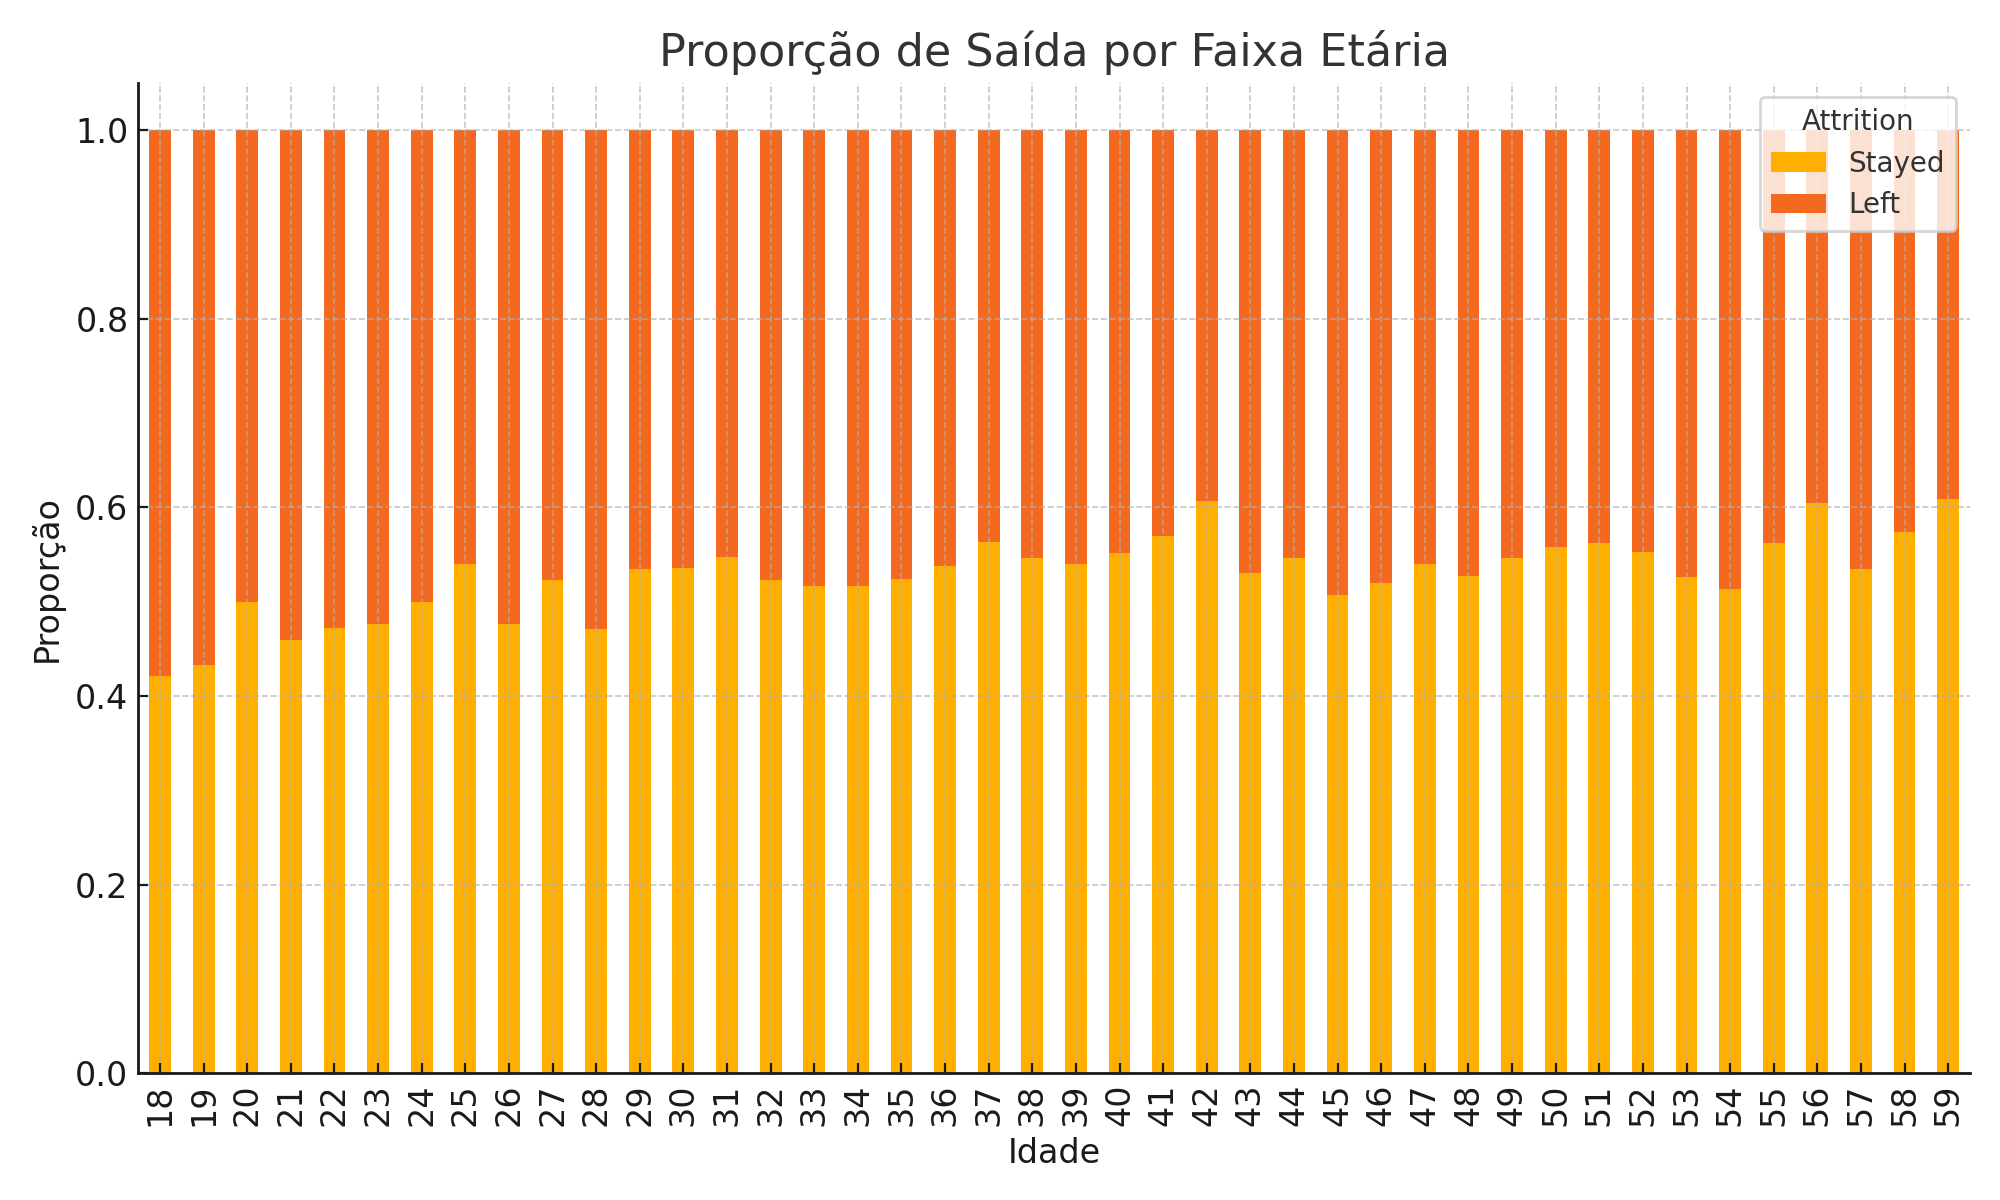
\includegraphics[width=\linewidth]{images/age_attrition_distribution.png}
    \caption{Proporção de saída por faixa etária. Cada barra empilhada mostra, para idades entre 18 e 59 anos, a fração de funcionários que permaneceram (\textit{Stayed}, amarelo) e que saíram (\textit{Left}, laranja) segundo o \textit{Synthetic Employee Attrition Dataset}. Observa-se ligeira maior incidência de desligamentos nas faixas mais jovens (18–30 anos) e redução gradual ao longo da carreira.}
    \Description{Gráfico de barras empilhadas indicando, para cada idade de 18 a 59 anos, a proporção de funcionários que ficaram e dos que saíram da empresa.}
\end{figure}

\begin{figure}[!htbp]
    \centering
    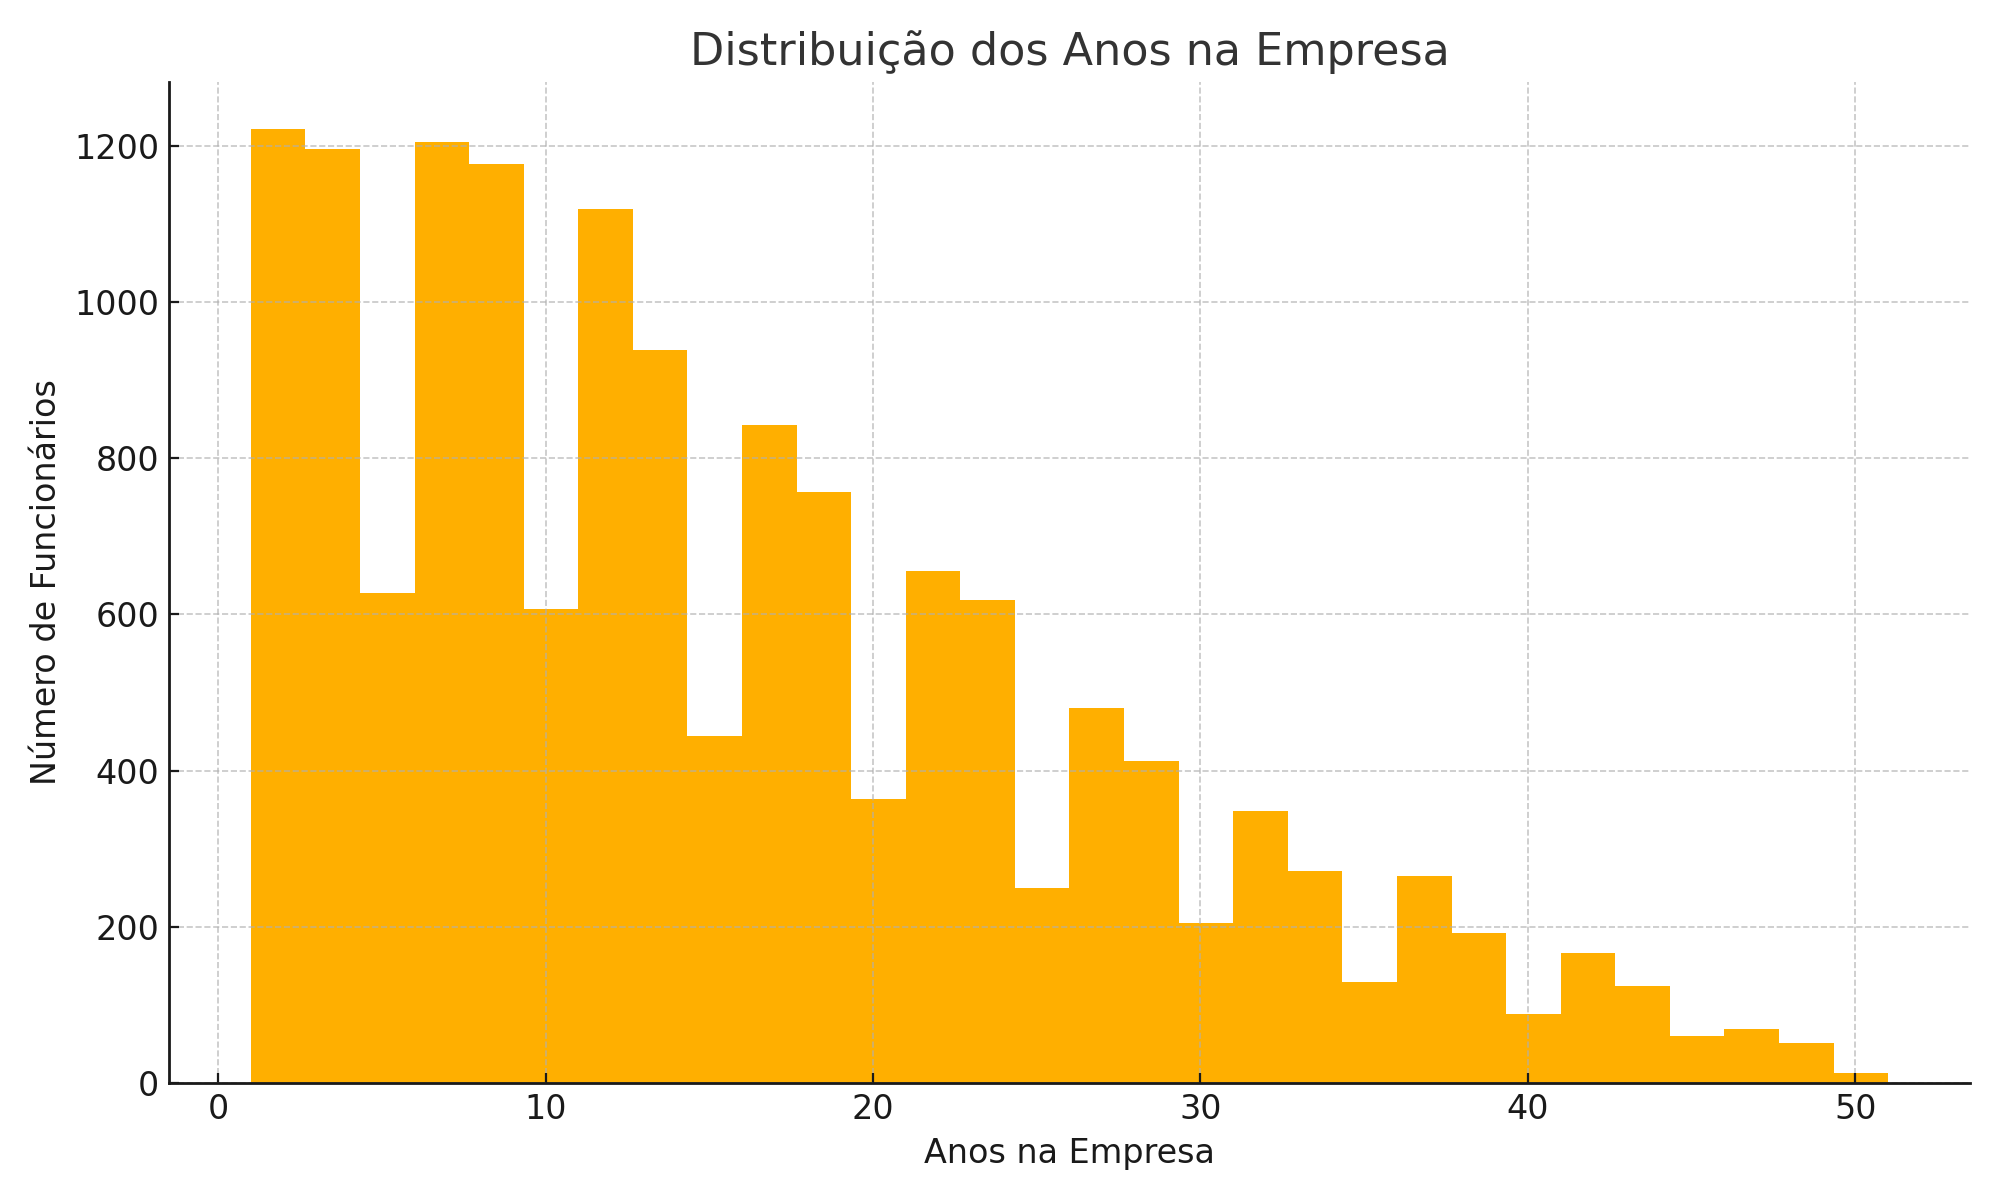
\includegraphics[width=\linewidth]{images/years_at_company_histogram.png}
    \caption{Distribuição dos anos na empresa. Histograma do atributo \textit{Years at Company}; a maioria dos colaboradores possui até 15 anos de casa, com número decrescente de casos conforme o tempo de empresa aumenta, evidenciando renovação de quadro.}
    \Description{Histograma em barras douradas mostrando a quantidade de funcionários para cada intervalo de anos na empresa, concentrada entre 0 e 15 anos.}
\end{figure}

\begin{acks}
Os autores agradecem à OpenAI ChatGPT pelo suporte na elaboração de trechos preliminares de texto e revisões linguísticas. Todo o conteúdo técnico, interpretação e conclusões são de responsabilidade exclusiva dos autores.
\end{acks}

\bibliographystyle{ACM-Reference-Format}
\begin{thebibliography}{9}

\bibitem{dataset2025}
StealthTechnologies. 2024.
\newblock Synthetic Employee Attrition Dataset.
\newblock Kaggle. Retrieved May 27, 2025 from
  \url{https://www.kaggle.com/datasets/stealthtechnologies/employee-attrition-dataset}

\end{thebibliography}

\end{document}